\chapter{Fonts}
\label{ch:fonts}

\section{Missing glyphs in Arabic fonts}

In order to see Arabic script properly, the font you are using must contain Arabic glyphs (characters).  A number of fonts developed especially for Arabic are available,\footnote{For example, in the Ubuntu packages \textit{fonts-arabeyes} or \textit{fonts-kacst}, or on the web from the Open Font Library (\url{openfontlibrary.org/en/search?query=Arabic}).} but many of them contain only the glyphs needed to write standard Arabic.

If you are using \textbf{Andika!} to transcribe older manuscripts, it may be that these glyphs will be all you need, since many Swahili writers in the past used the Arabic script to provide only an approximation to the Swahili sounds, and depended on the linguistic knowledge of native speakers to interpret the text correctly \citep[p14-15]{Omar2002}.\footnote{The examples are: \AS{نِغِمَا وَغُ بِنْتِ} (\textit{negema wangu binti}), \AS{يِيِ كِيَ مُولَ وَكُ} (\textit{nyenyekea Mola wako}), and \AS{مْتُ هُنِنَ اَكِرَ * اَسِيَابَرَكِ تَرَ} (\textit{mtu hunena akenda * asiyapanda kitanda})}  As a further example, a copy of stanza 6 of the \textbf{Utenzi wa Mwana Kupona} (\textit{Mwana Kupona's Ballad}), as written by Muhammad Kijuma (c.1855--1945),\footnote{MS H58, Asia Africa Institute/CSMC, University of Hamburg.} is given below:

\begin{figure}[h]
 \centering
 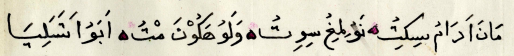
\includegraphics[keepaspectratio=true]{./images/mwanakuponas6.png}
 % mwana_kupona_s6.png: 514x56 pixel, 96dpi, 13.60x1.48 cm, bb=0 0 385 42
  \caption{Stanza 6 from Muhammad Kijuma's manuscript of \textit{Utenzi wa Mwana Kupona}}
 \label{fig:mwanakupona}
\end{figure}

The following is a letter-for-letter transcription of stanza 6, along with an automatically-generated close transliteration and a manually-added standard Roman transliteration and English translation:

\begin{longtable}[c]{rrl}
\textarabic{نَوُلِمِغُ سِوِتُ} & \textarabic{مَانَ اَدَامُ سِكِتُ} &  \textarabic{٦} \\* 
\Tr{nawulimiḡu siwiṯu} & \Tr{māna aḏāmu sikiṯu} & \Tr{6b/a} \\*
\multicolumn{2}{r}{\Swa{mwana adamu si kitu, na ulimwengu si wetu}} & \Tr{6a/b} \\* 
\multicolumn{2}{r}{\E{mankind is as nothing, and the world does not belong to us}} & \\ 
\textarabic{اَبَوُ اَتَسَلِيَا} & \textarabic{وَلَوُ هَكُوْنَ مْتُ} &  \\* 
\Tr{abawu aṯasaliya} & \Tr{walawu hakūna mṯu} & \Tr{6d/c} \\* 
\multicolumn{2}{r}{\Swa{walau hakuna mtu ambao atasaliya}} & \Tr{6c/d} \\* 
\multicolumn{2}{r}{\E{and there is no person who will live forever}} & \\ 
\end{longtable}

However, if you are not dealing solely with older manuscripts, and you wish to use the spelling conventions proposed in \textbf{Andika!} in order to unambiguously represent current-day Swahili, and allow transliteration between Arabic script and the standard Swahili Roman script, then you will need the additional glyphs.  If you see squares or boxes in the Arabic script, or just the glyph for the isolated form when initial, medial or final forms are required, the reason is that the font you are using is missing the glyphs that it would make it useable with Swahili.

The missing glyphs are likely to be one or more of those in \Cref{tab:missglyphs}.  The first seven glyphs are the most important.
\begin{table}[h!]
\centering
\begin{tabularx}{14cm}{llll}
\textbf{Glyph} & \textbf{Unicode name} & \textbf{Unicode number} & \textbf{Notes} \\
\hline\noalign{\smallskip}
\AS{پ} & peh & U+067E & \textbf{p} \\
\AS{ڤ} & veh & U+06A4 & \textbf{v} \\
\AS{چ} & tcheh & U+0686 & \textbf{ch} \\
\AS{ڠ} & ain with three dots above & U+06A0 & \textbf{g} \\
\AS{ݝ} & ain with two dots above & U+075D & \textbf{g} in \textbf{ng'} \\
\AS{ٖ} & subscript alef & U+0656 & short \textbf{e} \\
\AS{ٗ} & inverted damma & U+0657 & short \textbf{o} \\
\AS{\char"063B} & keheh with two dots above & U+063B & used by some writers for \textbf{ch} \\  % entering keheh from the keyboard won't work -- the codepoint seems not to be in Linux Biolinum
\AS{ٹ} & tteh & U+0679 & alveolar \textbf{t} (Mombasa) \\
\AS{ڈ} & ddal & U+0688 & alveolar \textbf{d} (Mombasa) \\
\AS{ۏ} & waw with dot above & U+06CF & \textbf{w} (North) \\
\AS{ژ} & jeh & U+0698 & \textbf{zh} (North) \\
\end{tabularx}
\caption{Glyphs commonly missing in fonts}
\label{tab:missglyphs}
\end{table}

At the time of writing, the only fonts which contain all of these additional glyphs in \Cref{tab:missglyphs} are Scheherazade\footnote{\url{scripts.sil.org/cms/scripts/page.php?item_id=Scheherazade}, available in the Ubuntu package \textit{fonts-sil-scheherazade}, but see also \Cref{s:fonts}.} (by Bob Hallissy and Jonathan Kew), Amiri\footnote{\url{amirifont.org}} (by Khaled Hosny), and the fonts from the PakType project.\footnote{\url{paktype.sourceforge.net}, available in the Ubuntu package \textit{fonts-paktype}.}

Fonts containing all the glyphs in \Cref{tab:missglyphs} apart from \textit{keheh} are Droid Arabic Naskh\footnote{\url{openfontlibrary.org/en/font/droid-arabic-naskh}} and Droid Arabic Kufi\footnote{\url{openfontlibrary.org/en/font/droid-arabic-kufi}} (by Pascal Zoghbi), and Lateef.\footnote{\url{scripts.sil.org/cms/scripts/page.php?item_id=Lateef}}

\section{Default fonts in \textbf{Andika!}}
\label{s:changefont}

When typing Swahili in Arabic script, the fonts can be changed directly in LibreOffice.  For typesetting of existing manuscripts,  \textbf{Andika!} uses four fonts as defaults when generating pdfs:
\begin{itemize}
\item Scheherazade for the Arabic transcription.  A possible alternative here is Amiri.
\item Linux Biolinum O\footnote{\url{linuxlibertine.org}} for the close transcription into Roman script, since it is especially good at handling diacritics.  A possible serif alternative here is Gentium\footnote{\url{scripts.sil.org/cms/scripts/page.php?site_id=nrsi&item_id=Gentium}} (by Victor Gaultney).
\item Liberation Serif\footnote{\url{fedorahosted.org/liberation-fonts}} for English translations.
\item GranadaKD in \textit{andika/fonts} for poem titles in Arabic.  This is a Kufic-style font from Arabeyes\footnote{\url{openfontlibrary.org/en/font/granada}} that has been adapted by me to add the characters in \Cref{tab:missglyphs} except \textit{keheh}.
\end{itemize}

These default fonts can be changed by replacing the name of the font in the relevant command in \textit{convert/tex/fontdefs.tex}.  Thus, to change the transliteration font from Linux Biolinum O to Gentium, you would first install Gentium:

\verb|sudo apt-get install fonts-sil-gentium|

and then open \textit{convert/tex/fontdefs.tex} in a text-editor\footnote{A text-editor is an application specialising in the editing of text.  Word-processors should never be used to edit files in \textbf{Andika!}, because they will quietly change the file in ways which will prevent it working.  There are multiple text-editors such as Kate, Geany, and Gedit available in Ubuntu.} and change the line:

\verb|\newcommand\Tr[1]{{\fontspec[Scale=1, Color=666666]{Linux Biolinum O}#1}}|

to:

\verb|\newcommand\Tr[1]{{\fontspec[Scale=1, Color=666666]{Gentium}#1}}|

The \textit{Color} command sets the colour of the font using the hex version of the RGB value\footnote{\url{colorspire.com/rgb-color-wheel}} (in this case, dark grey) -- delete it if you want the transliteration in black.  The \textit{Scale} command alters the size of the font -- if you want it a bit smaller than normal, enter (say) 0.8 instead of 1.

As a general point, the readability of diacritics (or even whether they are displayed at all) depends crucially on the font -- not all will be capable of showing all diacritics, or of placing them in the right location, so if something is not looking right in your transliteration, try using Linux Biolinum O (sans-serif) or Gentium (serif) as suggested. 

\section{Adding missing glyphs to Arabic fonts}

If you are anxious to use a particular Arabic font that does not have all the glyphs required by Swahili, it is possible to add them to the font using the font editor FontForge,\footnote{\url{fontforge.github.io}} originally developed by George Williams.  Appendix \ref{appB} shows how to use FontForge to add missing glyphs,\footnote{Note that unless the font you are adapting is available under an open license, this may constitute a breach of copyright.} and a version with screenshots is also available at the website for the book \textit{Design with FontForge}.\footnote{\url{designwithfontforge.com/en-US/Adding_Glyphs_to_an_Arabic_Font.html}}

You can also develop your own fonts using FontForge, though the creation of an attractive font is a highly specialised task requiring artistic flair as well as technical skill.   The next version of the drawing program Inkscape,\footnote{\url{inkscape.org}} 0.49, will allow initial glyph designs to be created there and then imported into FontForge for finalisation.\footnote{\url{understandingfonts.com/blog/2011/11/typography-extensions-in-inkscape-0-49}.  In the meantime, this functionality can be accessed by using the ``bleeding edge'' packages available from Inkscape Trunk -- \url{launchpad.net/~inkscape.dev/+archive/ubuntu/trunk}.}

\section{Scheherazade and Amiri}
\label{s:sham}

The Scheherazade webpage\footnote{\url{scripts.sil.org/cms/scripts/page.php?item_id=Scheherazade}} notes that:
\begin{quotation}
Scheherazade provides a “simplified” rendering of Arabic script, using basic connecting glyphs but not including a wide variety of additional ligatures or contextual alternates (only the required lam-alef ligatures). This simplified style is often preferred for clarity, especially in non-Arabic languages, but may not be considered appropriate in situations where a more elaborate style of calligraphy is preferred.
\end{quotation}

Scheherazade is the default in \textbf{Andika!} because it fits the proposed full vocalisation better.  For instance, Amiri places all the vowels at the same height from the main letter, eg \Am{كُبٗرٖيشَ} (\textit{kuboresha}, to boost) compared to Scheherazade \AS{كُبٗرٖيشَ}, and \Am{وَنَسَيَانْسِ} (\textit{wanasayansi}, scientists) compared to Scheherazade \AS{وَنَسيَانْسِ}. This can lead to the upper vowels from the current line of text colliding with the lower vowels from the previous line.

However, Amiri may be more appropriate for use with text that is not fully vocalised (eg quotation of Arabic within Swahili), particularly since it includes more of the ligatures commonly used in Arabic, making for more attractive text. For instance, Amiri \Am{وَلِتُمئَِ} (\textit{walitumia}, they used), compared to Scheherazade \AS{وَلِتُمئَِ}, has the letters \textit{ltm} combined in one ligature.
